
%----------- slide --------------------------------------------------%
\begin{frame}
\frametitle{AIRS deconvolution}
\begin{itemize}

  \item

  \item

  \item

\end{itemize}
\end{frame}
%----------- slide --------------------------------------------------%

\begin{column}{0.5\textwidth}
  \begin{centering}
  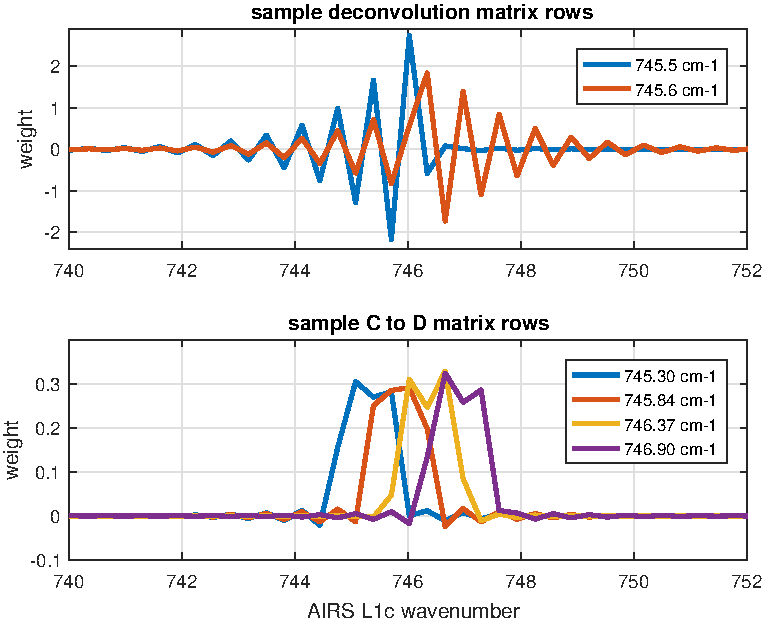
\includegraphics[width=\textwidth]{figures/airs_decon_basis.pdf}
  \end{centering}
  sample adjacent rows for the deconvolution and L1c to L1d
    transforms

\end{column}

%----------- slide --------------------------------------------------%
\begin{frame}
\frametitle{translation overview}
  \begin{centering}
  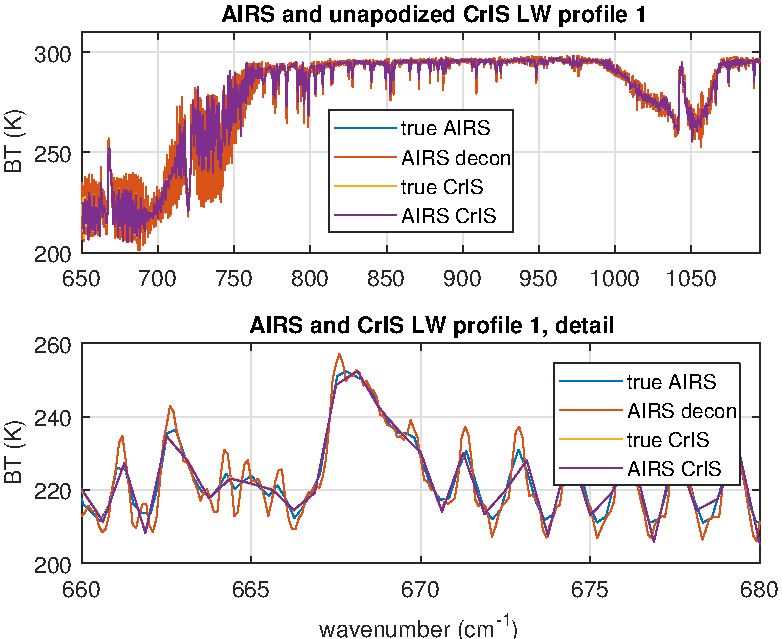
\includegraphics[width=0.8\textwidth]{figures/a2cris_spec_LW.pdf}
  \end{centering}
  true {\airs}, deconvolved {\airs}, true {\cris}, and {\airs}
  {\cris}.  Differences between true {\cris} and {\airs} {\cris} are
  too small to be visible in this figure.
\end{frame}

\begin{column}{0.5\textwidth}  
  \begin{centering}
  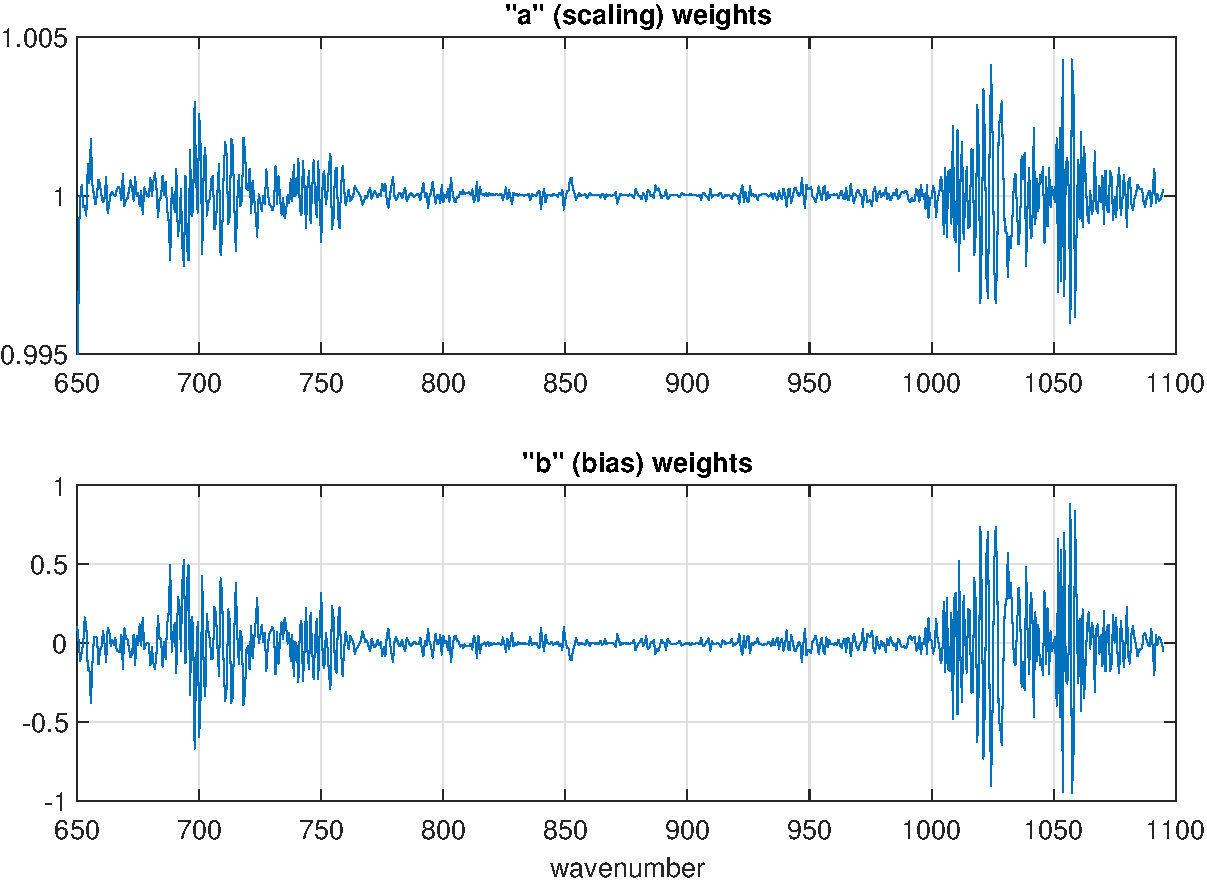
\includegraphics[width=\textwidth]{figures/a2cris_coef_LW.pdf}
  \end{centering}\vspace{3mm}
  LW $a$ and $b$ weights for the linear correction $ax+b$.

\end{column}

%----------- slide --------------------------------------------------%
\begin{frame} % source plot_SRF2.m
\frametitle{{\airs} spectral response functions}
\begin{center}
   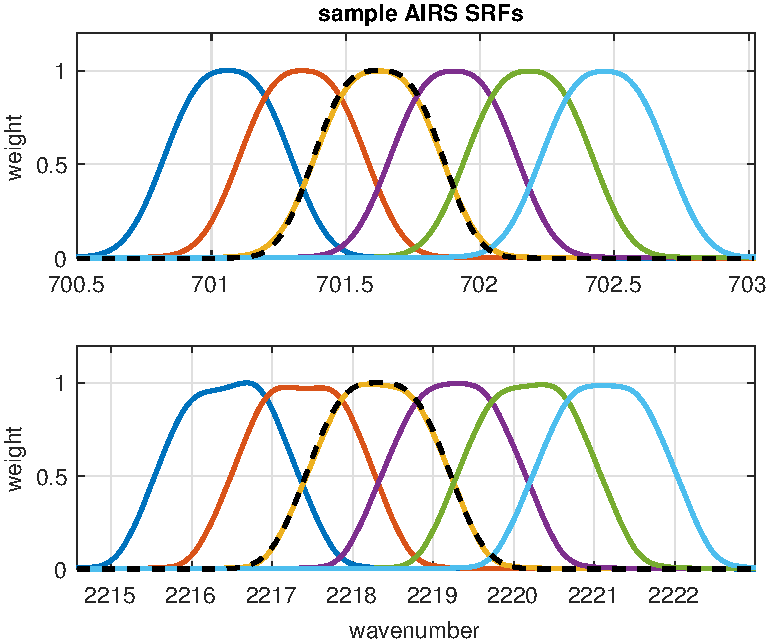
\includegraphics[width=0.6\textwidth]{figures/airs_sample_SRF.pdf}
 \end{center}
sample {\airs} spectral response functions from the low and high
ends of the band.  The dashed line is a generalized Gaussian
function.
\end{frame} 
%----------- slide --------------------------------------------------%
\begin{frame} % source plot_SRF2.m
\frametitle{channel spacing and resolving power}
\begin{center}
  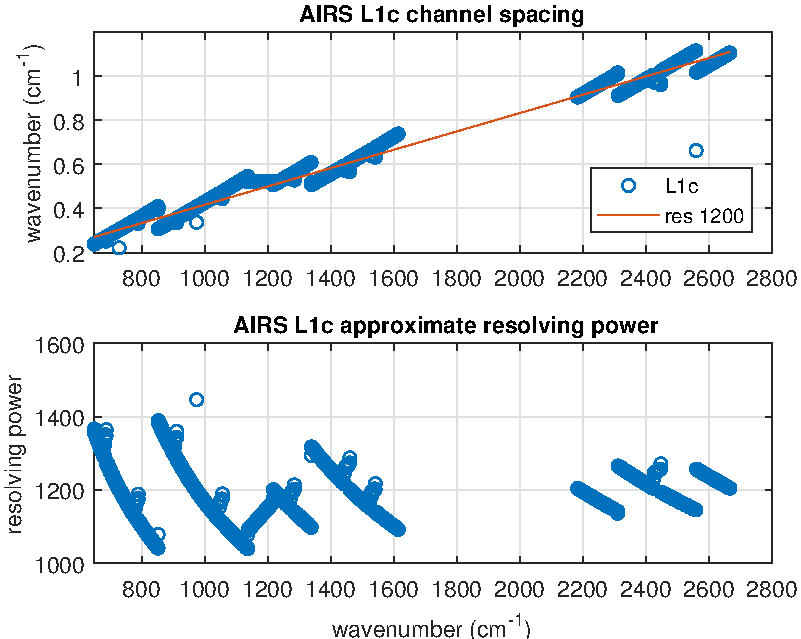
\includegraphics[width=0.9\textwidth]{figures/airs_L1c_res.pdf}
\end{center}
% {\airs} L1c channel spacing and derived resolving power
\end{frame} % source plot_subpt.m
%----------- slide --------------------------------------------------%
\begin{frame}
\frametitle{channel spacing and resolving power}
\begin{columns}[t]
\begin{column}{0.5\textwidth}

\end{column}
\begin{column}{0.5\textwidth}  

\end{column}
\end{columns}
\end{frame}
%----------- slide --------------------------------------------------%
\begin{frame} % source plot_SRF2.m
\frametitle{channel spacing and resolving power}
\begin{columns}[t]
\begin{column}{0.5\textwidth}
  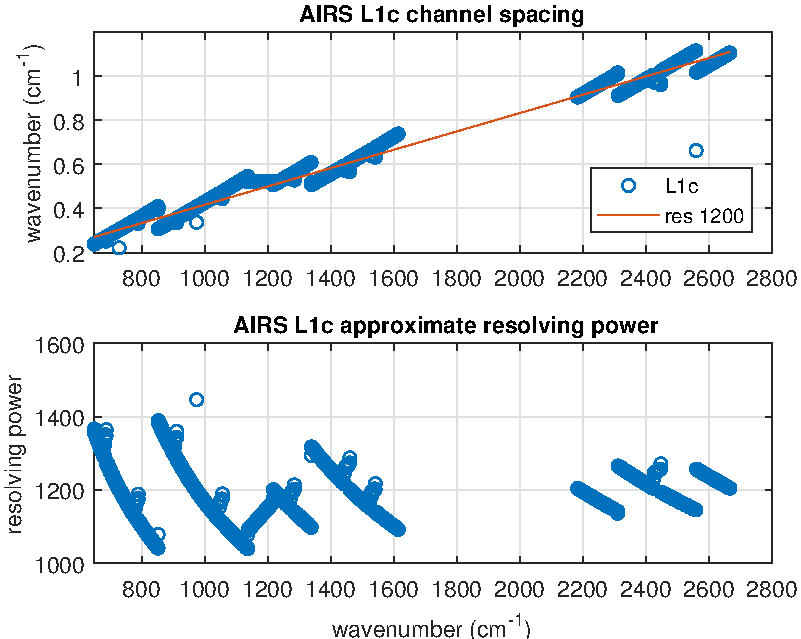
\includegraphics[width=\textwidth]{figures/airs_L1c_res.pdf}
  \begin{itemize}
     \item some text here some text here some 
     \item some text here some text here some 
  \end{itemize}

\end{column}
\begin{column}{0.5\textwidth}  
    \begin{center}
      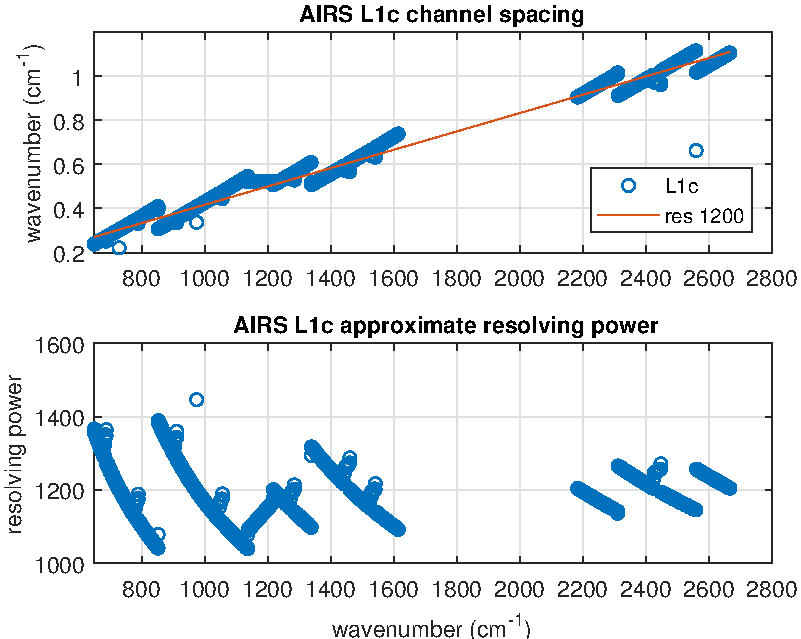
\includegraphics[width=\textwidth]{figures/airs_L1c_res.pdf}
     \end{center}
text here some text here some text here sample {\airs} spectral
response functions from the low and high ends of the band.  The
dashed line is a generalized Gaussian function.
\end{column}
\end{columns}
\end{frame} % source plot_subpt.m
%%----------- slide --------------------------------------------------%
\begin{frame} % source plot_SRF2.m
\frametitle{channel spacing and resolving power}
\begin{columns}[t]
\begin{column}{0.5\textwidth}

 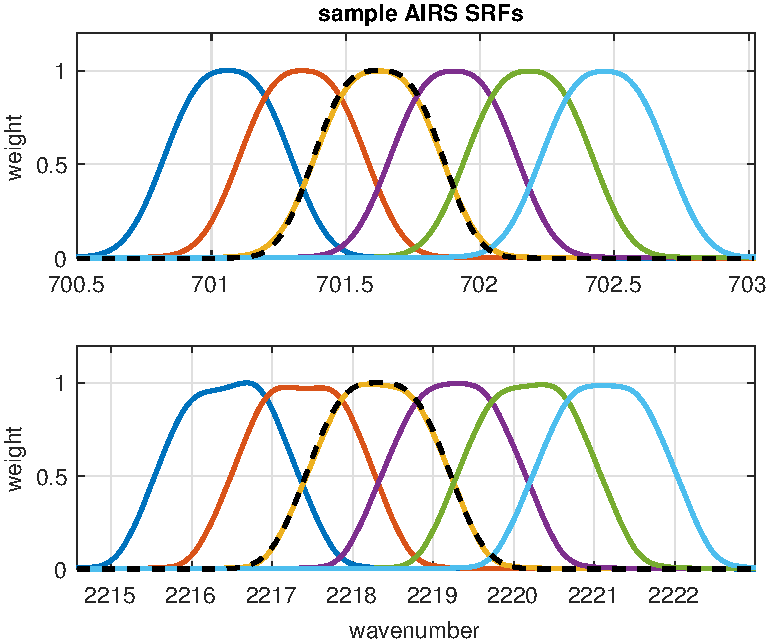
\includegraphics[width=\textwidth]{figures/airs_sample_SRF.pdf}

  sample {\airs} spectral response functions from the low and high
  ends of the band.  The dashed line is a generalized Gaussian
  function.

\end{column}
\begin{column}{0.5\textwidth}  
We chose a generalized Gaussian 
\cite{wiki:gauss} of the form
\[w(v, v_0, \fwhm) = 
\exp\left(-\left(\frac{(v - v_0)^2}{2c^2}\right)^{1.5}\right) \]
where $c=\fwhm / (2\sqrt{2\ln 2})$ and $v_0$ is the desired channel
center.  
\end{column}
\end{columns}
\end{frame} % source plot_subpt.m
%%----------- slide --------------------------------------------------%
\begin{frame} % source plot_SRF2.m
\frametitle{channel spacing and resolving power}

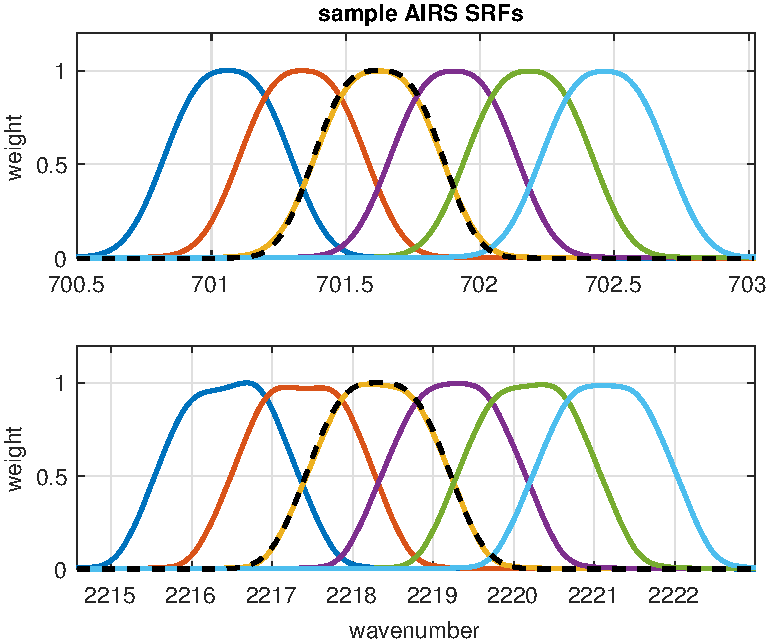
\includegraphics[width=0.5\textwidth]{figures/airs_sample_SRF.pdf}

sample {\airs} spectral response functions from the low and high
ends of the band.  The dashed line is a generalized Gaussian
function.  We chose a generalized Gaussian of the form
\[w(v, v_0, \fwhm) = 
\exp\left(-\left(\frac{(v - v_0)^2}{2c^2}\right)^{1.5}\right) \]
where $c=\fwhm / (2\sqrt{2\ln 2})$ and $v_0$ is the desired channel
center.  
\end{frame} % source plot_subpt.m
